\documentclass[screen, authorversion, nonacm, sigconf]{acmart}

\usepackage[linesnumbered,commentsnumbered,ruled]{algorithm2e}
\usepackage{graphicx}
\usepackage{booktabs}
\usepackage{tabularx}

\begin{document}

\title{Exploring the Impact of Decision Tree Depth}

\author{Alic Szecsei}
\affiliation{University of Iowa}
\email{alic-szecsei@uiowa.edu}

\author{Diego Castaneda}
\affiliation{University of Iowa}
\email{diego-castaneda@uiowa.edu}

\author{Willem DeJong}
\affiliation{University of Iowa}
\email{willem-dejong@uiowa.edu}

\begin{abstract}
  For classification problems, decision trees are a very easily understandable machine learning tool that does not require much computation to use after construction. However, they are easily susceptible to overfitting. A common means to combat this problem is by pruning the decision tree, according to some metric. While this is commonly chosen to be a $\chi^2$ analysis, a computationally trivial metric is simply the height of the decision tree. When a decision tree reaches a specified height, the construction algorithm constructs a leaf node. The process of model selection is designed to determine the optimal height of the decision tree while avoiding overfitting; the impact of tree height on this model selection process varies wildly from one dataset to another. We used four datasets from the UCI Machine Learning Repository and trained a decision tree learning algorithm on them to analyze the accuracies of the resulting decision trees. We determined that the datasets for which the decision tree process works best are those which have several unrelated attributes; datasets with interconnected attributes require much larger trees and tend to have higher error rates.
\end{abstract}

%% The code below is generated by the tool at http://dl.acm.org/ccs.cfm.
\begin{CCSXML}
  <ccs2012>
  <concept>
  <concept_id>10010147.10010257</concept_id>
  <concept_desc>Computing methodologies~Machine learning</concept_desc>
  <concept_significance>500</concept_significance>
  </concept>
  <concept>
  <concept_id>10010147.10010257.10010258.10010259.10010263</concept_id>
  <concept_desc>Computing methodologies~Supervised learning by classification</concept_desc>
  <concept_significance>300</concept_significance>
  </concept>
  <concept>
  <concept_id>10010147.10010257.10010293.10003660</concept_id>
  <concept_desc>Computing methodologies~Classification and regression trees</concept_desc>
  <concept_significance>300</concept_significance>
  </concept>
  <concept>
  <concept_id>10010147.10010257.10010339</concept_id>
  <concept_desc>Computing methodologies~Cross-validation</concept_desc>
  <concept_significance>100</concept_significance>
  </concept>
  </ccs2012>
\end{CCSXML}

\ccsdesc[500]{Computing methodologies~Machine learning}
\ccsdesc[300]{Computing methodologies~Supervised learning by classification}
\ccsdesc[300]{Computing methodologies~Classification and regression trees}
\ccsdesc[100]{Computing methodologies~Cross-validation}

\keywords{decision trees, model selection}

\maketitle

\section{Background and Motivation}

Machine learning algorithms fall into one of two categories: classification and regression. In regression, input data is consumed and transformed by a function which can produce values along a numeric range; in classification, data is categorized into a finite number of possible values, and machine learning algorithms seek only to label data sets. These classification problems can use both numeric and categorical data attributes. For purely categorical data, decision trees are a way to build machine learning algorithms that are understandable by both humans and machines. Rather than a sort of ``black box'' in which numbers are passed in and answers are returned, there is a logical tree hierarchy that is familiar to anyone who has played the game Twenty Questions.

Decision trees require both a way to construct them, and a way to use them to categorize data. This categorization is a trivial tree traversal, and so many of the innovations regarding decision trees have to do with their construction. Most decision tree construction algorithms use a two-phase approach: first a \emph{growing} phase, followed by a \emph{pruning} phase. In the growing phase, the decision tree is built out, trying to fit the provided training data as closely as possible. To combat over-fitting, the pruning phase commonly uses $\chi^2$ tests to determine which branches of the tree are too ``noisy'' and removes them.

Additionally, decision tree models can be constrained by size to combat overfitting. Russell and Norvig \cite{russell_norvig_2010} showcase an implementation of restricting a decision tree to be beneath a maximum size by generating the tree in breadth-first fashion, and stopping when the maximum number of nodes has been reached. As stated in Garofalakis, Hyun, Rastogi, and Shim \cite{Garofalakis:2000:EAC:347090.347163}, there is no point in creating a branch when it is guaranteed to be pruned later.

The amount of pruning which occurs is heavily dependent on the data set chosen. As such, the exact values which optimize our trained decision trees are relatively unimportant. However, our goal was to examine how impactful depth-based pruning was, and how much it assisted with reducing overfitting.

\section{Methods}

\subsection{Dataset Selection}

Our first step was selecting the datasets to use as the foundation for our programs. We used four UCI data sets \cite{Dua:2019}:

\begin{enumerate}
  \item \texttt{MUSHROOMS}, a dataset to classify mushrooms as edible or inedible
  \item \texttt{BALANCE}, a dataset to classify whether or not a scale with objects of varying weights and distances was balanced
  \item \texttt{CAR}, a dataset of car evaluations
  \item \texttt{TICTACTOE}, a dataset of Tic-Tac-Toe board states classified as to whether or not `x' will win.
\end{enumerate}

These datasets were selected as they have a variety of both number of attributes and number of examples. \texttt{MUSHROOMS} has 8124 examples with 22 attributes, for example, while \texttt{BALANCE} only has 625 examples and 5 attributes. In addition, some of our datasets were calculated from synthetic data, while others were from real-world data collection. We tried to choose a diverse selection of datasets so that our algorithm testing results would not be overly skewed towards certain types of datasets.

\subsection{Decision Tree Generation}

The foundation of our decision tree algorithm is the one provided by Russell and Norvig \cite{russell_norvig_2010} which, in turn, is based on the ID3 algorithm \cite{Quinlan1986}.

\begin{function}
	\SetAlgoLined
  \SetKwFunction{PluralityValue}{Plurality-Value}
  \SetKwFunction{Importance}{Importance}
  \caption{DecisionTreeLearning($examples$, $attributes$, $parent\_examples$, $depth$)}
  \label{algo:DecisionTreeLearning}
  \uIf{$examples$ is empty}{\Return{\PluralityValue{$parent\_examples$}}}
\uElseIf{$depth = 0$}{\Return{\PluralityValue{$examples$}}}
  \uElseIf{all $examples$ have the same classification $c$}{\Return{a leaf node $c$}}
  \ElseIf{$attributes$ is empty}{\Return{\PluralityValue{$examples$}}}
  $A \gets argmax_{a \in attributes} \Importance{a, examples}$\;
  $tree \gets$ a new decision tree with root test $A$\;
  \ForEach{value $v_k$ of $A$}{
    $exs \gets \left\{e : e \in examples \text{ and } e.A = v_k\right\}$\;
    $subtree \gets \DecisionTreeLearning{exs, attributes - A, examples, depth - 1}$\;
    add a branch to $tree$ with label $\left(A = v_k\right)$ and subtree $subtree$\;
  }
  \Return{$tree$}\;
\end{function}

A two-stage approach was used: first, a decision tree generator was developed, which we named \texttt{dtl}. This program would take in a flag as a command-line argument to determine which of our data sets was represented by the input. As the order of the attributes and classes varied between datasets, we were able to use these flags to significantly simplify the process of importing data by hardcoding in this information. 

\subsection{Classification}

A second program, \texttt{classify}, was used to classify data using a decision tree generated from \texttt{dtl}. This program takes in two arguments: the first is a path to a learned decision tree and the second is a path to the corresponding dataset to classify. To enable \texttt{classify} to traverse a decision tree generated by \texttt{dtl}, a JSON representation of the decision tree was used. This data format allowed us to produce human-readable representations of these decision trees, which we could use as a sanity check during the development process. \texttt{classify} is also used heavily in the $k$-fold cross-validation process, which was used to validate our generated models.

\subsection{External Packages}

To assist with the command-line interface, we used the \texttt{cmdliner} module. This allowed us to define data types and arguments for input, and \texttt{cmdliner} handled the majority of the command-line parsing. \texttt{cmdliner} also automatically generated a \texttt{--help} option to inform users of what the different options for the programs were. This significantly simplified developing optional new features, as we could add an optional flag and \texttt{cmdliner} would handle parsing it.

Additionally, we used the \texttt{adtgen} module to generate a JSON serializer and deserializer. This was done at the very start of the project, which allowed us to work with and visualize decision tree data early in the development process. This also meant that as our decision tree model was updated and changed, the JSON serialization and deserialization code was automatically shared between \texttt{dtl} and \texttt{classify} and the two programs were consistently in sync.

\subsection{$k$-fold Cross-Validation}

Finally, we split $k$-fold cross-validation into two implementations. The first, done in Python, was very simple to get working; we were able to start collecting data fairly early on in the development process. Simultaneously, we developed a model selection program in OCaml, which used a similar cross-validation algorithm to the one in the Python script. This model selection program performed $k$-fold cross-validation at maximum depth levels ranging from 1 to 10 and selected the result with the lowest error values, returning the decision tree generated at that depth for further use.

Using Python to generate data for $k$-fold cross-validation allowed us to collect data from both our decision tree program, \texttt{dtl}, as well as the decision tree algorithm provided by scikit-learn \cite{scikit-learn}. This provided a simple baseline comparison for our experimentation.

We then ran each of our datasets through the \ref{algo:DecisionTreeLearning} algorithm implemented in \texttt{dtl}, with maximum depths ranging from 1 to 10 and performed $k$-fold cross-validation to determine error rates, with $k = 4$. We noticed that subsequent experiments could obtain dramatically varying error rates, and so we repeated each of these experiments for 100 trials, and determined average error rates and their variances.

\section{Results}

The results of our experimentation varied between datasets. For \texttt{MUSHROOMS} in particular, our algorithm was able to achieve significantly greater accuracy than scikit-learn for smaller maximum depth constraints (figure \ref{fig:mushoursvscikit}). However, for other datasets, such as \texttt{TICTACTOE}, our algorithm produced consistently more error-prone results at all depth values (figure \ref{fig:tttoursvscikit}).

\begin{figure}
  \centering
  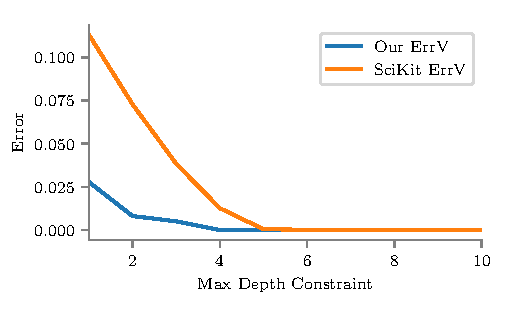
\includegraphics[width=\columnwidth]{figures/chart_ours_v_scikit_mushrooms.pdf}
  \caption{Error for our algorithm versus scikit-learn on the \texttt{MUSHROOMS} dataset}
  \label{fig:mushoursvscikit}
  \Description{A rapidly decreasing graph, with our algorithm starting at around $2.5$ percent error and dropping to near-zero, and scikit-learn starting at around $10$ percent error and dropping to similar levels at a depth of $5$.}
\end{figure}

\begin{figure}
  \centering
  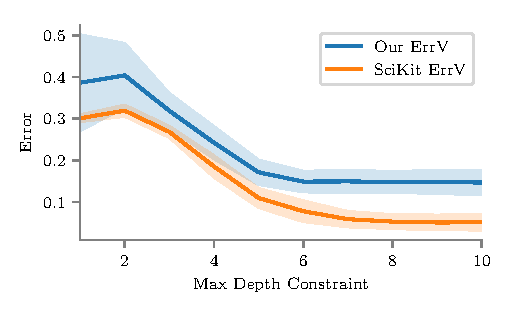
\includegraphics[width=\columnwidth]{figures/chart_ours_v_scikit_variance_tictactoe.pdf}
  \caption{Error ($\pm 2 \times SD$) for our algorithm versus scikit-learn on the \texttt{TICTACTOE} dataset}
  \label{fig:tttoursvscikit}
  \Description{A graph in which both our algorithm and that of scikit-learn are approximately parallel. Ours starts at approximately $40$ percent error and drops to $20$ percent at depth five, while scikit-learn starts at approximately $30$ percent and drops to less than $10$ percent at depth 8.}
\end{figure}

The \texttt{CAR} dataset proved to be the most interesting. While our algorithm had worse accuracy than scikit-learn for small depth values, as the maximum permitted depth increased we began to outperform scikit-learn's algorithm (figure \ref{fig:caroursvscikit}).

\begin{figure}
  \centering
  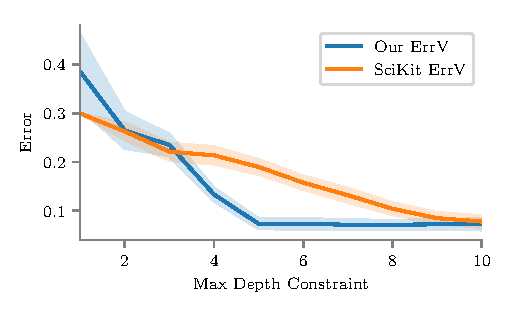
\includegraphics[width=\columnwidth]{figures/chart_ours_v_scikit_variance_car.pdf}
  \caption{Error ($\pm 2 \times SD$) for our algorithm versus scikit-learn on the \texttt{CAR} dataset}
  \label{fig:caroursvscikit}
  \Description{A graph in which our error starts at around $40$ percent and drops to less than $10$ percent at depth five; scikit-learn takes until depth $9$ to reach a similar level, despite it starting at $30$ percent.}
\end{figure}

\section{Discussion}

Overall, we found that our DecisionTreeLearning algorithm performed much worse on datasets with a large amount of interconnected data, such as Tic-Tac-Toe. This may be because, in these problems, an attribute's impact is heavily dependent on all of the other attributes in the data set. For more independent classification problems, such as evaluating cars or mushrooms, our DecisionTreeLearning algorithm was very accurate.

One of the concerns in decision tree learning is overfitting. From our results, we saw that the only dataset we started overfitting on was \texttt{TICTACTOE}. This was likely due to the datasets we chose having significant complexity; although \texttt{BALANCE} had the fewest attributes, its classifications relied on combinations of all of them. Our simplest datasets also used synthetic data calculations to provide examples, reducing the amount of noise present in the data; the more complex models were the ones gathered from real-world data and so were at the most risk of overfitting - but the number of attributes was so high that a maximum depth of 10 didn't appear to reach an optimal model selection value.

We were surprised at the discrepancies between our DecisionTreeLearning algorithm and the one provided by scikit-learn, as we expected both decision tree algorithms to produce similar results. While an effort was made to impose similar constraints on both algorithms (scikit-learn was used with the ``entropy'' heuristic, as well as the same tree depth constraint), there were a few differences that we were unable to resolve. First, scikit-learn uses ``an optimised version of the CART \cite{DBLP:books/wa/BreimanFOS84} algorithm.''

Additionally, scikit-learn could not be used with categorical data. To get around this restriction, we used one-hot encoding for the scikit-learn algorithm. This encoding constructs new columns for each possible value in a categorical data column; these new columns are assigned a value of 1 if the row matches this category, and 0 otherwise. A naive approach of mapping categories to a range of numbers produces biased results, as this imposes an invalid numerical interpretation on the data. One-hot encoding sidesteps this issue by only using boolean values of 0 and 1. Unfortunately, this one-hot encoding caused a negative impact on the depth: scikit-learn's decision tree was forced to be a binary tree, meaning it could not contain as many nodes as our trees for a given depth. Depth constraints thus had more of an impact on scikit-learn than they did on our DecisionTreeLearning algorithm.

The algorithm used by scikit-learn resulted in much closer variance than ours; however, scikit tended to maintain a constant variance, while our DecisionTreeLearning algorithm decreased in variance as we increased the maximum depth of the tree. This indicated to us that while scikit-learn's algorithm produced consistently good results for most datasets, our algorithm could produce both much better or much worse results for those same datasets.

For future work, we would like to make the \texttt{dtl} algorithm more generalized. Rather than inputting a specific flag to use hardcoded data, providing a more extensible interface for users other than ourselves. Additionally, we would be able to more closely emulate scikit-learn's functionality by using one-hot encoding for both our DecisionTreeLearning algorithm and scikit-learn. This could provide a more comparable baseline comparison.

We would also like to implement $\chi^2$ pruning to examine how using both or either of these pruning methods impacts average error.

\section{Role Assignment \& Contributions}

\subsection{Alic}

Alic was responsible for implementing the decision tree learning algorithm, the JSON decision tree representation, helped improve the binary executables, and implemented unit testing for several core functions. He implemented the decision tree learning algorithm from Russell and Norvig \cite{russell_norvig_2010}, and added an optional depth constraint. He also was responsible for constructing both the internal decision tree representation and determining the JSON representation for communicating between the \texttt{dtl} and \texttt{classify} binaries. Additionally, he improved the binary executable command-line experience, enabling order-independent options as well as a \texttt{--help} option. He wrote unit tests for core functions such as \texttt{Plurality-Value}, \texttt{Entropy}, and \texttt{DecisionTreeLearning} itself. Additionally, he was the lead writer on this technical report. He was the project checker.

\subsection{Willem}

Willem worked primarily on decision tree creation, data file read in, and model selection in OCaml. He created a data reader for CSV files, which was used by all of the OCaml binaries (\texttt{dtl}, \texttt{classifier}, and the OCaml-based model selection program). He helped program the \texttt{dtl} executable, which reads in a data file for the training data, then creates a decision tree. He also wrote up hard coded large amounts of information about the different sets of data, including information about the attributes, their possible values, the possible classification, etc. He also created the OCaml version of model selection using $k$-fold cross-validation, which takes in various optional and required command line arguments and prints out the selected tree, error rate in the training set, error rate in the validation set, and the chosen max depth. He also elected to be the project recorder.

\subsection{Diego}

Diego's primary focus was on writing and testing the classifier specified in the project specification. In developing the \texttt{classify} binary executable, Diego had to use OCaml's I/O functionality as well as methods generated from \texttt{adtgen} to read in the decision tree to be used for classification. Additionally he made use of the reader methods developed by Willem in order to get a list of examples to classify. As he developed the classifier he suggested that indexes referring to attributes be added as a field to the decision tree structure as it was necessary for pullling the correct attribute from an example. Diego also wrote tests using the OUnit testing framework. For testing the classifier, he mocked up sample trees and examples for some of the selected datasets and some made up scenario sets, and verified that the classifier was indeed classifying examples correctly. Lastly, as the designated coordinator he set up daily meetings in the engineering building, and checked to make sure everyone knew both their tasks and everyone else's.

%% The acknowledgments section is defined using the "acks" environment
%% (and NOT an unnumbered section). This ensures the proper
%% identification of the section in the article metadata, and the
%% consistent spelling of the heading.
\begin{acks}
This work was supported in part by the University of Iowa.
\end{acks}

\bibliographystyle{ACM-Reference-Format}
\bibliography{tech-report}

\appendix

\section{Supplemental Graphs \& Data}

\begin{table*}
  \centering
  \begin{tabular}{lrrrrrrrr}
    \toprule
    {} & \multicolumn{2}{c}{\texttt{BALANCE}} & \multicolumn{2}{c}{\texttt{CAR}} & \multicolumn{2}{c}{\texttt{MUSHROOMS}} & \multicolumn{2}{c}{\texttt{TICTACTOE}} \\
    \cmidrule(r){2-3} \cmidrule(lr){4-5} \cmidrule(lr){6-7} \cmidrule(l){8-9} 
    MaxDepth &     Avg Error & SD &     Avg Error & SD &     Avg Error & SD &     Avg Error & SD \\
    \midrule
    1        &  0.404191 &           0.012534 &  0.299769 &       6.409876e-17 &  0.113245 &       6.927670e-17 &  0.301035 &           0.004068 \\
    2        &  0.359704 &           0.019186 &  0.262998 &       8.538287e-03 &  0.072871 &       6.937492e-17 &  0.319115 &           0.006669 \\
    3        &  0.299806 &           0.013906 &  0.221366 &       8.831223e-03 &  0.038405 &       3.836886e-17 &  0.268329 &           0.006638 \\
    4        &  0.253065 &           0.012958 &  0.213860 &       8.886552e-03 &  0.012629 &       1.224688e-04 &  0.185432 &           0.012746 \\
    5        &  0.227718 &           0.011899 &  0.190035 &       7.656538e-03 &  0.000446 &       1.144321e-04 &  0.110016 &           0.011334 \\
    6        &  0.235505 &           0.011984 &  0.157795 &       6.878887e-03 &  0.000137 &       1.420214e-04 &  0.078250 &           0.012445 \\
    7        &  0.234140 &           0.011871 &  0.131944 &       7.268610e-03 &  0.000027 &       9.986264e-05 &  0.059186 &           0.009237 \\
    8        &  0.227516 &           0.011412 &  0.104103 &       6.179355e-03 &  0.000025 &       9.896975e-05 &  0.053361 &           0.008296 \\
    9        &  0.224897 &           0.010037 &  0.084815 &       5.794818e-03 &  0.000022 &       8.814005e-05 &  0.051273 &           0.008884 \\
    10       &  0.222565 &           0.009456 &  0.077986 &       5.976894e-03 &  0.000016 &       7.951336e-05 &  0.051618 &           0.009168 \\
    \bottomrule
  \end{tabular}
  \caption{Errors and standard deviations of decision trees for different datasets}
  \label{tab:errs}
\end{table*}

\begin{figure}[H]
  \centering
  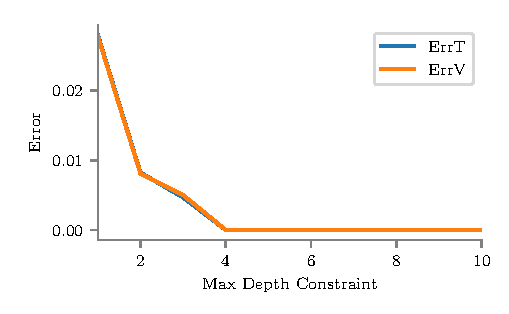
\includegraphics[width=\columnwidth]{figures/chart_errt_errv_mushrooms_ours.pdf}
  \caption{The error on training and validation data for the \texttt{MUSHROOMS} data set}
  \label{fig:mushroomserrterrv}
\end{figure}

\begin{figure}[H]
  \centering
  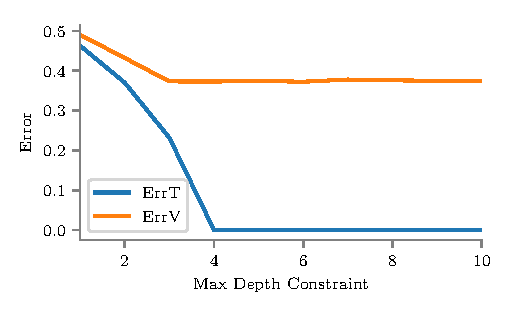
\includegraphics[width=\columnwidth]{figures/chart_errt_errv_balance_ours.pdf}
  \caption{The error on training and validation data for the \texttt{BALANCE} data set}
  \label{fig:balanceerrterrv}
\end{figure}

\begin{figure}[H]
  \centering
  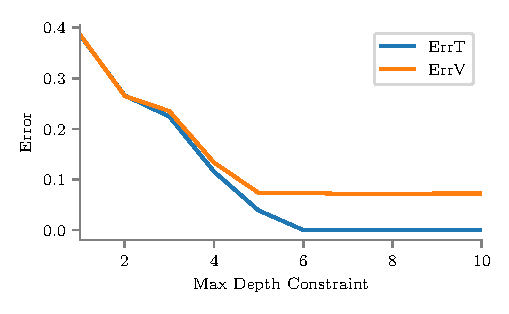
\includegraphics[width=\columnwidth]{figures/chart_errt_errv_car_ours.pdf}
  \caption{The error on training and validation data for the \texttt{CAR} data set}
  \label{fig:carerrterrv}
\end{figure}

\begin{figure}[H]
  \centering
  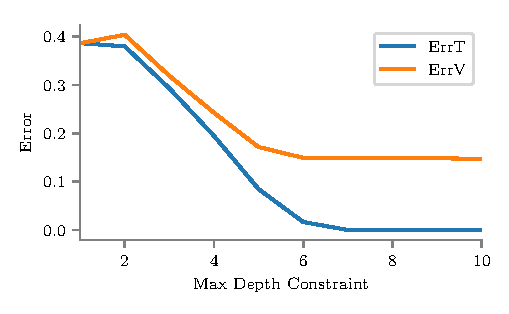
\includegraphics[width=\columnwidth]{figures/chart_errt_errv_tictactoe_ours.pdf}
  \caption{The error on training and validation data for the \texttt{TICTACTOE} data set}
  \label{fig:ttterrterrv}
\end{figure}

\end{document}
\endinput